\documentclass[11pt, twocolumn]{article}

% GRAPHICS
\usepackage{float}
\usepackage{graphicx}
\usepackage{subcaption}

% HYPERLINKS
\usepackage{hyperref}

% DOCUMENT PADDING AND MARGINS
\usepackage{titlesec}
\usepackage[margin=0.8in]{geometry}
%\setlength{\parskip}{\baselineskip}%
%\setlength{\parindent}{0pt}
\titlespacing*{\section}{0pt}{2ex}{0ex}
\titlespacing*{\subsection}{0pt}{2ex}{0ex}
\titlespacing*{\subsubsection}{0pt}{2ex}{0ex}

% COMMENTING
\usepackage{comment}

% MATH FONTS
\usepackage{amsmath}


\begin{document}

% TITLE
\title{Autonomous Quadrotor Landing on a Moving Platform}
\author{Stan Brown \& Chris Choi}
\date{}
\maketitle

\section{Introduction}
Over the years there has been a growing interest in autonomous landing of quadrotors, as landing is often one of the most dangerous and risk prone parts of flight. There are now several commercial and research based implementations of autonomous landing with both the DJI Phantom and Pixhawk flight controllers being capable of automatic landing using a series control algorithms. However, there does not appear to be a reliable method of landing a quadrotor on either a moving platform or in relatively large wind disturbances. 

In recent years. there have been at least least 5 academic publications on the topic \cite{Lee2012, Kim2014, Voos2010, Friis2009, Ling2014, Herisse2012} that approach the problem from a variety of angles. Overall none of these approach have completely solved the problem and most approaches only work on slow moving platforms with little or no wind disturbances. 

One of the most challenging problems associated with autonomous landing is the difficulty of obtaining a reliable state estimate of the landing target relative to the quadrotor. This is due to the fact that the landing target can often go out of the camera's field of view causing the quadrotor to lose track of the target or measurements can become corrupted by vision based artifacts that include lighting, lens distortion, color, etc. In many cases GPS is not a viable option both the landing target and the quadrotor due a lack of accuracy unless an RTK GPS system is used. In many cases the use of an RTK system is not a readily available option due to cost and the lack of required equipment. 

\subsection{Related Work}
The autonomous landing problem can be thought of as a set of three separate control problems or stages. First the quadrotor must detect the relative position and velocity of the landing target using either GPS of visual methods. Next the quadrotor must determine a rendezvous location with the landing target and plan the required flight trajectory. Once the quad has rendezvoused a final landing trajectory must be calculated between quadrotor and the landing pad. 

For the perception portion of the problem there have been two main techniques use to identify the landing pad and estimate its state relative to the quadrotor. In the work of Kim, 2014 \cite{Kim2014} a basic color thresholding technique was used to identify the landing target and the MIT AprilTags library \cite{apriltags} was used to provide state estimations. In the work of Heriesse Et al. \cite{Herisse2012} an optical flow technique was applied to a series of images captured on-board the quadrotor to estimate the required states required to control the quadrotor and conduct autonomous landing. While both of these techniques have been shown to work in very specific cases both, require case specific parameters to be applied ahead of time, thereby limiting there general applicability. 

In the case of Ling \cite{Kim2014}, the brightness used in his thresholding technique must be set ahead of time and is sensitive to lighting changes. A similar issue is noted in the work of Heriesse \cite{Herisse2012}. Moreover in the work of Lim, there are also implementation issues due to the slow state estimation rate of the AprilTag library and, the AprilTag falling out of view of the camera during the final stages of decent. This meant that as the quadrotor approach the landing pad, it tended to lose any measurements of its state and therefore had complete the final landing procedure by propagating the last measured state forward in time. 

From the controls perspective the majority of literature either uses a set of PID or a Linear Quadratic Controller (LQC) controllers to command and control the quadrotor at all stages of flight based on the state estimation provided by the techniques discussed above. An LQC was thoroughly explored in Friis Et al. \cite{Friis2009} but the authors admit even though LQC performed slightly better than the PID controller the difference was minor and may be attributed to the additional time spent tuning the LQC. In \cite{Herisse2012}, a PID controller was developed to land on a vertically oscillating platform no lateral movement. While interesting, the solution took over 1 minute to transition from hovering over the landing pad to landing. Additionally the experiments did not seem to account for pitch or roll of the platform. 

In this project we focus developing a set of controllers that produce the final landing trajectory and using a  AprilTags \cite{apriltags} to provide the estimated state of the quadrotor relative to the landing pad. We seek to develop both a more robust and rapid method of determining the state of the quadrotor and landing pad system and to develop a set of PID controllers that can be used to control the quadrotor based on the measured state information.

\section{Methodology}
This project was be separated into two individual, but complementary components. First, a significant effort was spent on ensuring the quadrotor's state was estimated at a rate of at least 20 Hz with AprilTags. Secondly, using information from the estimated quadrotor state, a state machine and a PID position controller were developed to track and lands on a desired target.

\subsection{Measurement and State Estimation using AprilTags}
\label{subsec:AprilTag}
One of the challenges faced when estimating the quadrotor state using AprilTags was the computational resources required to sustain a rate of atleast 20 Hz. This problem was also noted in the work of \cite{Ling2014} where he addressed the issue by reducing the brightness of the image so that the majority of the image is black except for the AprilTag, thus reducing image processing requirements. An example of this implementation is shown in Figure~\ref{fig:ling_apriltags}. This allowed Ling \cite{Lee2012} to calculate states at a rate of approximately 10 - 15 Hz, but it came at the cost of requiring the brightness parameters to be set ahead of time and also the removed a large portion of robustness techniques normally included in the AprilTag library.

\begin{figure}[H]
	\centering
	\begin{subfigure}[b]{0.45\linewidth}
		\includegraphics[width=\textwidth]{images/ling_apriltags_1.png}
	\end{subfigure}
	\begin{subfigure}[b]{0.45\linewidth}
		\includegraphics[width=\textwidth]{images/ling_apriltags_2.png}
	\end{subfigure}
	\caption{Ling's approach to optimizing AprilTags detection \cite{Ling2014}}
	\label{fig:ling_apriltags}
	\vspace{-0.4cm}
\end{figure}

In this work, the slow rate of state estimation was addressed using three novel ideas. First, the image size and calibration parameters are set depending on the distance between the quadrotor's position relative to the AprilTag. Secondly, we introduce the use of a Region of Interest (ROI) window to focus only on the AprilTag to reduce computational time required to estimate the pose. Thirdly, we embed a smaller AprilTag into a larger one that is used to provide state estimates when the distance to the landing pad is quite small (2 meters). 

\subsubsection{Adaptive Image Preprocessing}
As discussed previously, the low rate of the AprilTag library when processing images of 640 by 480 pixels results in an update rate of approximately 3 to 5 fps on the small on-board computers used on the target quadrotor, which is too low to be utilized effectively in a PID controller. Building upon the work of \cite{Ling2014}, who improved the AprilTag estimation rate by reducing the brightness on the image such that the majority of the pixels are black.

\subsubsection{Adaptive Image Windowing}
If one assumes that the quadrotor does not move too fast, there is relativity low rotation between captured images, and the image update rate is quite fast (60 fps in this implementation), then the location the AprilTag in the following image can be estimated based off of the location it was last observed in the previous image. Therefore whenever an AprilTag is measured in an image, a bounding box around the AprilTag is calculated and then used in the following image to blackout out portions of the image where the AprilTag is unlikely to be. An example of this implementation is highlighted in Figure \ref{fig:apriltags_windowing}. In cases where the AprilTag is not observed in the expected location (bounding box), the size of the bounding box is set to the size of the image and the entire image is processed. 

\begin{figure}[H]
	\centering
	\begin{subfigure}[b]{0.45\linewidth}
		\includegraphics[width=\textwidth]{images/apriltags_roi_1.png}
	\end{subfigure}
	\begin{subfigure}[b]{0.45\linewidth}
		\includegraphics[width=\textwidth]{images/apriltags_roi_2.png}
	\end{subfigure}
	\caption{Adaptive Image Windowing}
	\label{fig:apriltags_windowing}
\end{figure}

While the adaptive windowing procedure decreases the computational resources needed for extracting pose estimates, there are two additional problems that windowing cannot solve. First, as the size of the observed Apriltag increases, windowing is no longer adequate in decreasing computational time, this is an issue in cases where a high update rate is required (e.g. quadrotor landing). Second, as the observed AprilTag gets larger it becomes easy for the camera to lose track of the AprilTag itself, increasing the risk of no estimation for that time. Both of these problems are addressed by embedding a smaller AprilTag into the larger one.

\subsubsection{AprilTag Inception}
To address both the decreasing state update rate as a function of proximity and reduce the probability of losing sight of the AprilTag during landing a secondary AprilTag is embedded in the larger AprilTag, we term this technique AprilTag Inception (patent pending). This secondary AprilTag is assigned different family ID to avoid confusion during detection, and is placed at the center of the larger primary AprilTag. Whenever the secondary AprilTag is captured in the image, the adaptive windowing method is set to track only the secondary AprilTag rather than the larger one, which reduces the portion of the image that must be processed in with each image capture. An example of this procedure is highlighted in Figure \ref{fig:apriltagInception}.
 
\begin{figure}[H]
	\centering
	\begin{subfigure}[b]{0.45\linewidth}
		\includegraphics[width=\textwidth]{images/apriltags_1.png}
		\caption{2 Apriltags Detected}
	\end{subfigure}
	\begin{subfigure}[b]{0.45\linewidth}
		\includegraphics[width=\textwidth]{images/apriltags_3.png}
		\caption{1 Apriltag Detected }
	\end{subfigure}
	\caption{Apriltag Inception }
	\label{fig:apriltagInception}
\end{figure}

\subsubsection{Adaptive Image Down-sampling}
The final technique used to optimize the AprilTag detection was the introduction of down sampling the image size as the estimated distance between camera and AprilTag decreased. In this work two image down sampling sizes $320 \times 280$ (half resolution) and $160 \times 140$ (quarter resolution), were used. Whenever the distance between the camera and the AprilTag is less than 1.5 and 3 meters, the images are down sampled to the two resolutions respectively. If the camera is further than 3 meters from the AprilTag, the native resolution of $640 \times 480$ is used. This change only affected the image processing time when the quadrotor is within 3 meters of the quad and has the desired effect of maintaining a high AprilTag estimation rate.


\subsection{Controller and State Monitoring}
\label{subsec:position_controller}
In this project it is assumed that the quadrotor has successfully rendezvoused with the target vehicle and has a clear view through the camera image of the landing target located on the target vehicle at all times. The first step in autonomous landing is to position the quadrotor above the landing target such that the displacements in the x and y directions in the horizontal plane normal to the landing surface are near zero while simultaneously matching speed and aligning the axis with the target vehicle. Next, while maintaining the near zero displacements in the x and y directions, the quadrotor must descend at a safe rate such that the vertical distance between the quadrotor and the landing target is reduced until landing is achieved. Ideally the quadrotor will descend rapidly when the vertical displacement between the qaudrotor and target is large, slowing down just above ($\approx 1m$) the landing target to minimize time and energy requirements of the landing manoeuvre. 

To achieve the described behaviour, a set of PID position controllers were developed that output attitude commands such as roll and pitch to reduce the horizontal and vertical distance between the quadrotor and the landing platform, along with an altitude command to maintain a safe approach altitude such that the target does not go out of view during landing. Yaw control is omitted in the following work and is assumed to be axis aligned with the direction of travel of the moving target at all stages of decent and tracking. 

The derived position controller takes the quadrotor's desired position and current position in $x$, $y$ and $z$ of the world frame as inputs, which are then mapped to attitude and altitude commands in the roll $\hat{\phi_t}$, pitch $\hat{\theta_t}$ and thrust $\hat{T_z}$ relative to the quadrotor frame as outlined in Equations \ref{eq:pid_roll}, \ref{eq:pid_pitch}, \ref{eq:pid_thrust}, these equations as written assume that yaw $\psi$ is 0. In the case that the yaw is non-zero, then roll and pitch need to be adjusted to account for the yaw changes as in Equation \ref{eq:pid_roll_adjusted} and \ref{eq:pid_pitch_adjusted}. The altitude command is adjusted when roll $\hat{\phi}$ and pitch $\hat{\theta}$ are non-zero to maintain altitude as in Equation \ref{eq:pid_thrust_adjusted}. 

\begin{equation}
	\label{eq:pid_error}
	e = e_{\text{setpoint}} - e_{\text{actual}}
\end{equation}

\begin{equation}
	\label{eq:pid_roll}
	\hat{\phi_t} = K_p e_x + K_i \sum_{t = 0}^{t} e_{x, t} dt + K_d \dot{e}_{x,t}
\end{equation}

\begin{equation}
	\label{eq:pid_pitch}
	\hat{\theta_t} = K_p e_y + K_i \sum_{t = 0}^{t} e_{y,t} dt + K_d \dot{e}_{y ,t}
\end{equation}

\begin{equation}
	\label{eq:pid_thrust}
	\hat{T_z} =
		K_p e_z + K_i \sum_{t=0}^{t} e_{z,t} dt + K_d \dot{e_z}_{,t} 
\end{equation}

\begin{equation}
	\label{eq:pid_roll_adjusted}
	\phi_t = \cos(\psi_t) \hat{\phi_t} - \sin(\psi_t) \hat{\theta_t}
\end{equation}

\begin{equation}
	\label{eq:pid_pitch_adjusted}
	\theta_t = \sin(\psi_t) \hat{\phi_t} + \cos(\psi_t) \hat{\theta_t}
\end{equation}

\begin{equation}
	\label{eq:pid_thrust_adjusted}
	T = 
		T_{\text{hover}} +
		\frac{\hat{T_{z}}}{cos(\phi_t) cos(\theta_t)}
\end{equation}

\section{Results}
The methods outlined in sections \ref{subsec:AprilTag} and \ref{subsec:position_controller} were implemented and tested on real quadrotor with an onboard computer and camera. The quadrotor is assembled from a DJI F450 quadrotor frame, 4 Emax 2213-935KV motors with complementary DJI E310 420S 20A electronic speed controllers. A Pixhawk v2.4 running the PX4 firmware stack was selected for the flight controller and an Odroid XU4 was used as an on-board computer to processes process video captured from a using a PointGrey Firefly 2.0 camera operating 60 frames per second (fps) with a resolution of 640 by 480 pixels through a FuijiFilm 135 degree FOV lens. The camera calibration was done using the ROS camera calibration package. 

Images captured from the video stream are then processed using the AprilTag library after passing through the preprocessing steps outlined in \ref{subsec:AprilTag} and the estimated state is used by the PID controller (outlined in \ref{subsec:position_controller} and also running on the Odroid) to produce attitude commands that cause the quadrotor to move towards a goal location. All attitude commands are send to the Pixhawk from the Odroid via usb and rely heavily on the Mavros package, which is a wrapper around the popular Mavlink communication protocol. 

Using this testbed both the accuracy of the AprilTag state estimation was evaluated in the following sections. At this point in time a motion capture system was used in place of the AprilTag library to provide state estimates as it was found to be more reliable for initial testing purposes. In the coming week the PID controllers will also be tested using only the state estimates from the AprilTag library. 


\begin{figure}[H]
	\centering
	\includegraphics[width=0.8\linewidth]{images/quadrotor.jpg}
	\caption{DJI F450 with Pixhawk v2.4}
	\label{Quadrotor}
\end{figure}

\subsection{Evaluation of AprilTag Accuracy and Update Rate}
To evaluate the accuracy of the AprilTag and effects that the adaptive windowing procedures have on the state estimations an Optitrack motion capture system (MOCAP) was used to provide a ground truth. By monitoring the pose of both the camera and the AprilTag in the MOCAP system, the series of measurements were taken using the MOCAP system to calculate the pose of the AprilTag relative to the camera from a variety of ranges and angles. A comparison between the estimated pose from the AprilTag and the MOCAP system as a function of distance is highlighted in Figure \ref{fig:AprilTag_eval}. Figure \ref{fig:AprilTag_eval} also highlights the rate at which state estimates are received from the AprilTag library after being passed through the adaptive windowing procedure. A demo of the AprilTag pose estimation can also be seen in this 
\href{https://www.youtube.com/watch?v=BBMlQphrqCY&index=19&list=PLk5z6lLnKFd6BD9EXWa09hqf6SNQhn59R}{video}.

\begin{figure}	
	\centering
	\begin{subfigure}[b]{\linewidth}
		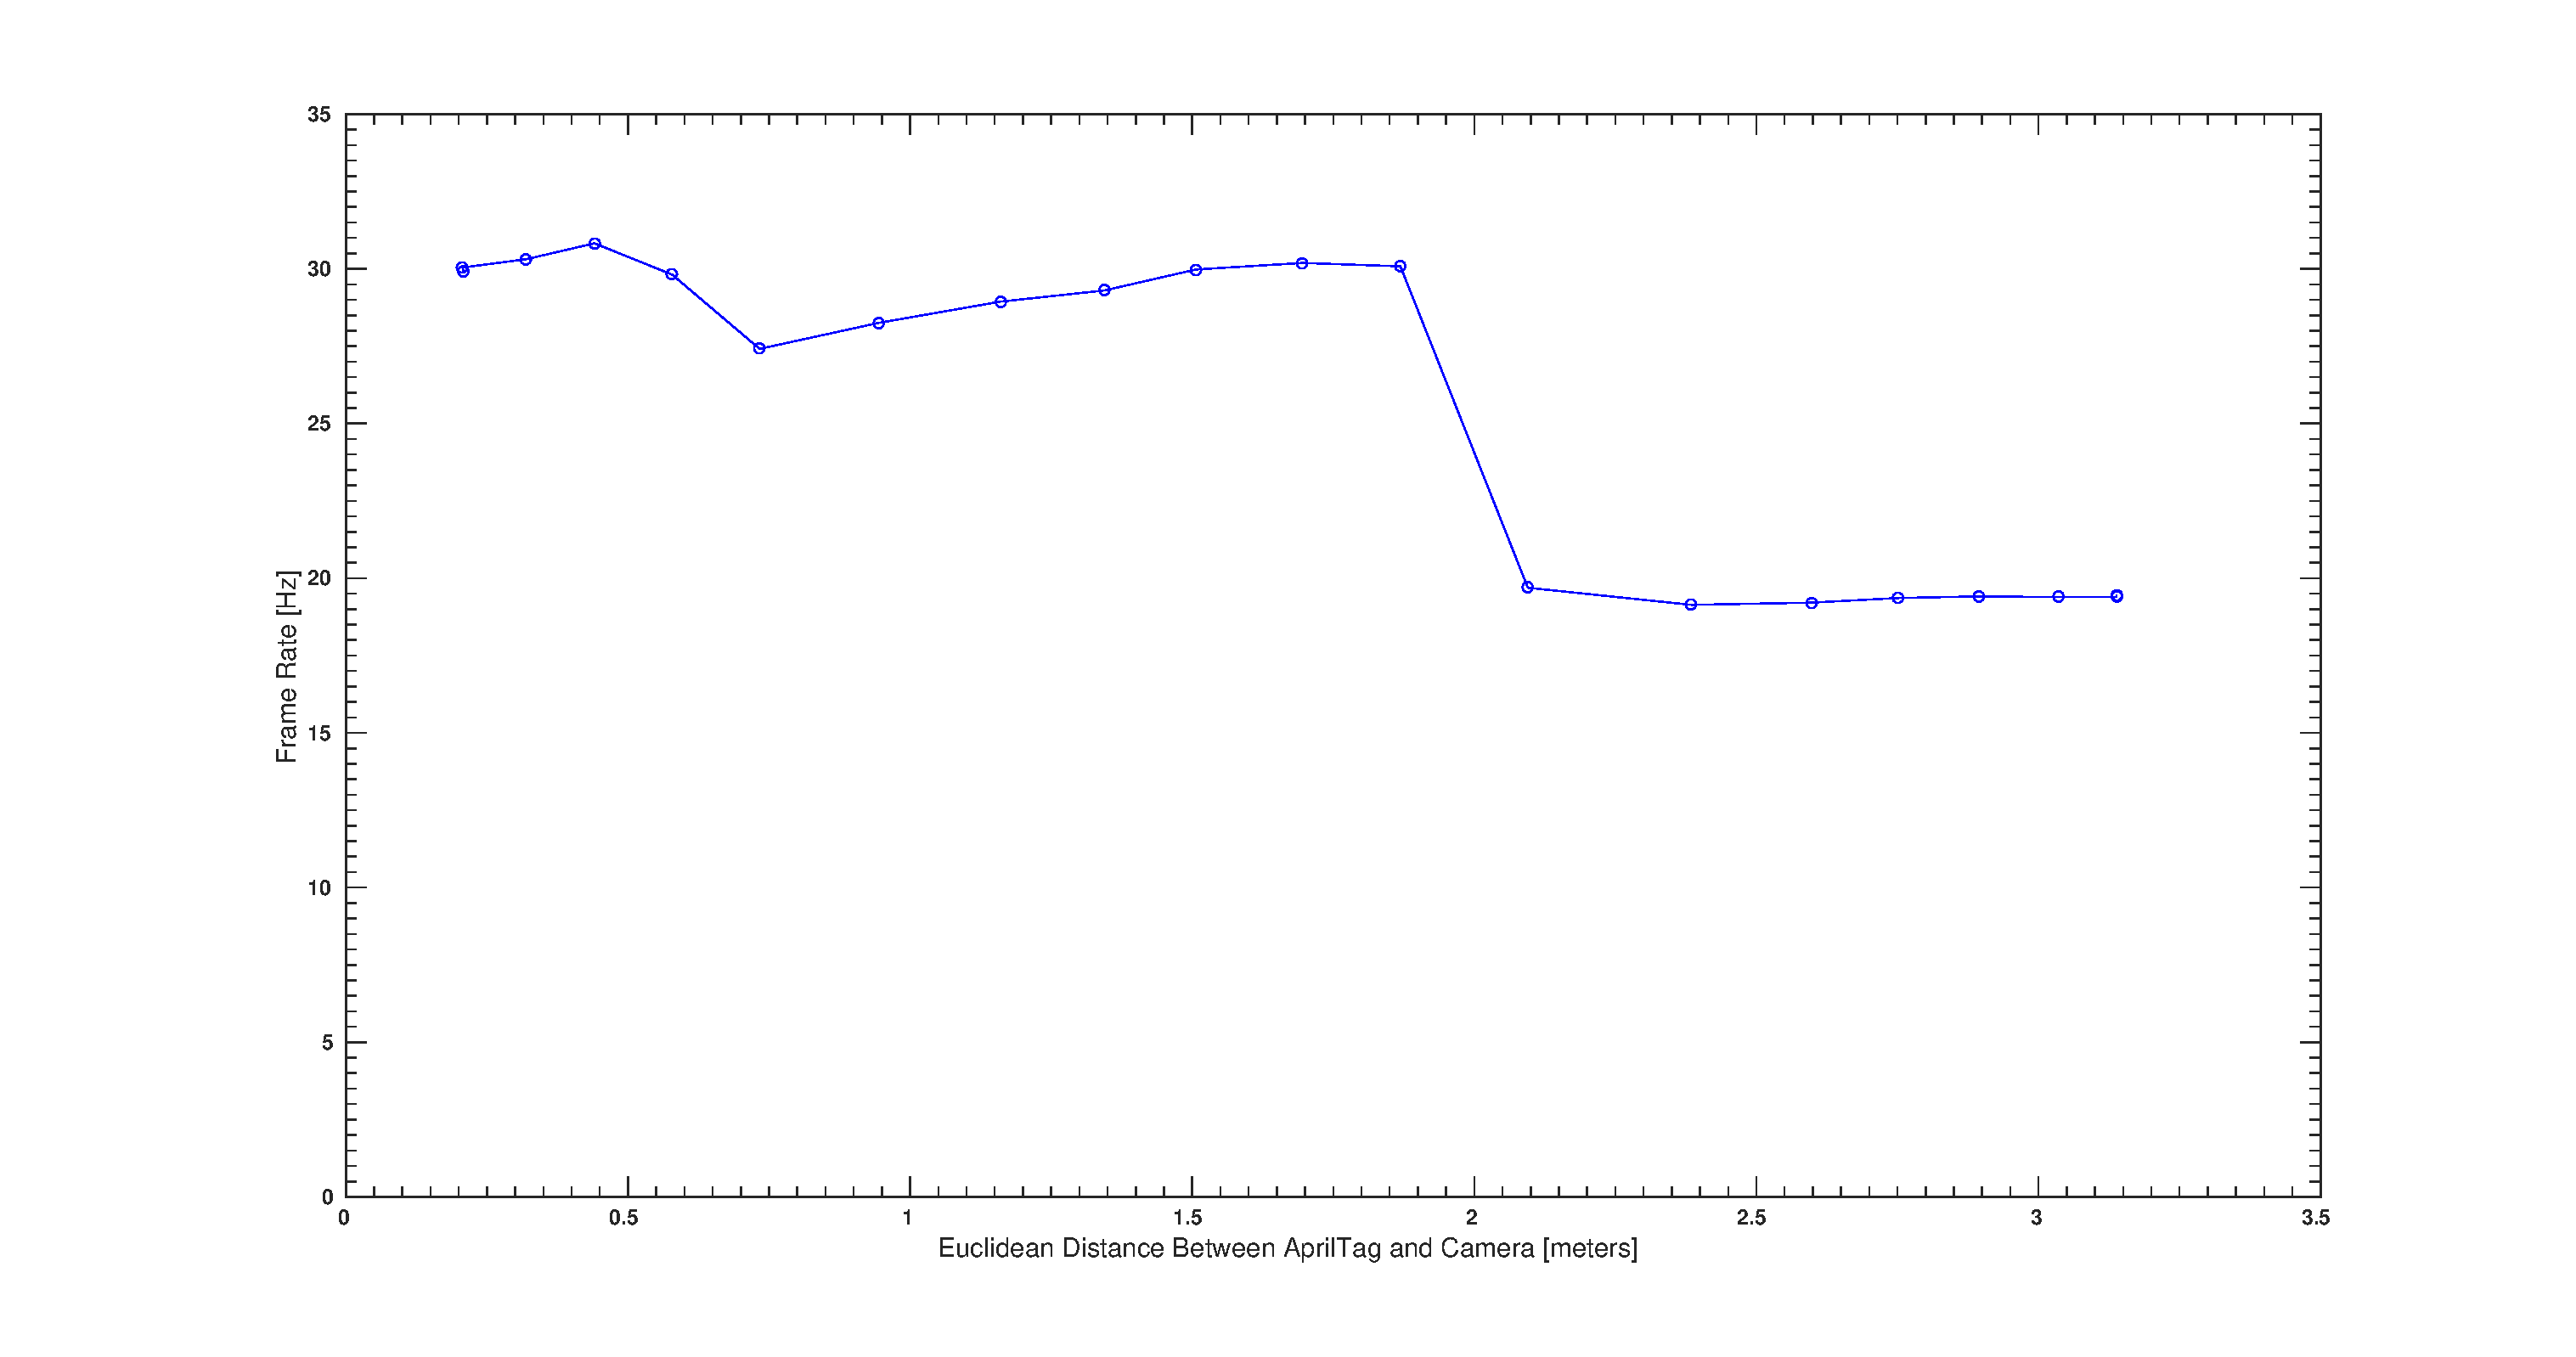
\includegraphics[width=\textwidth]{images/Apr_FPS_vs_Dist.eps}
		\caption{}
		
	\end{subfigure}

	\begin{subfigure}[b]{\linewidth}
		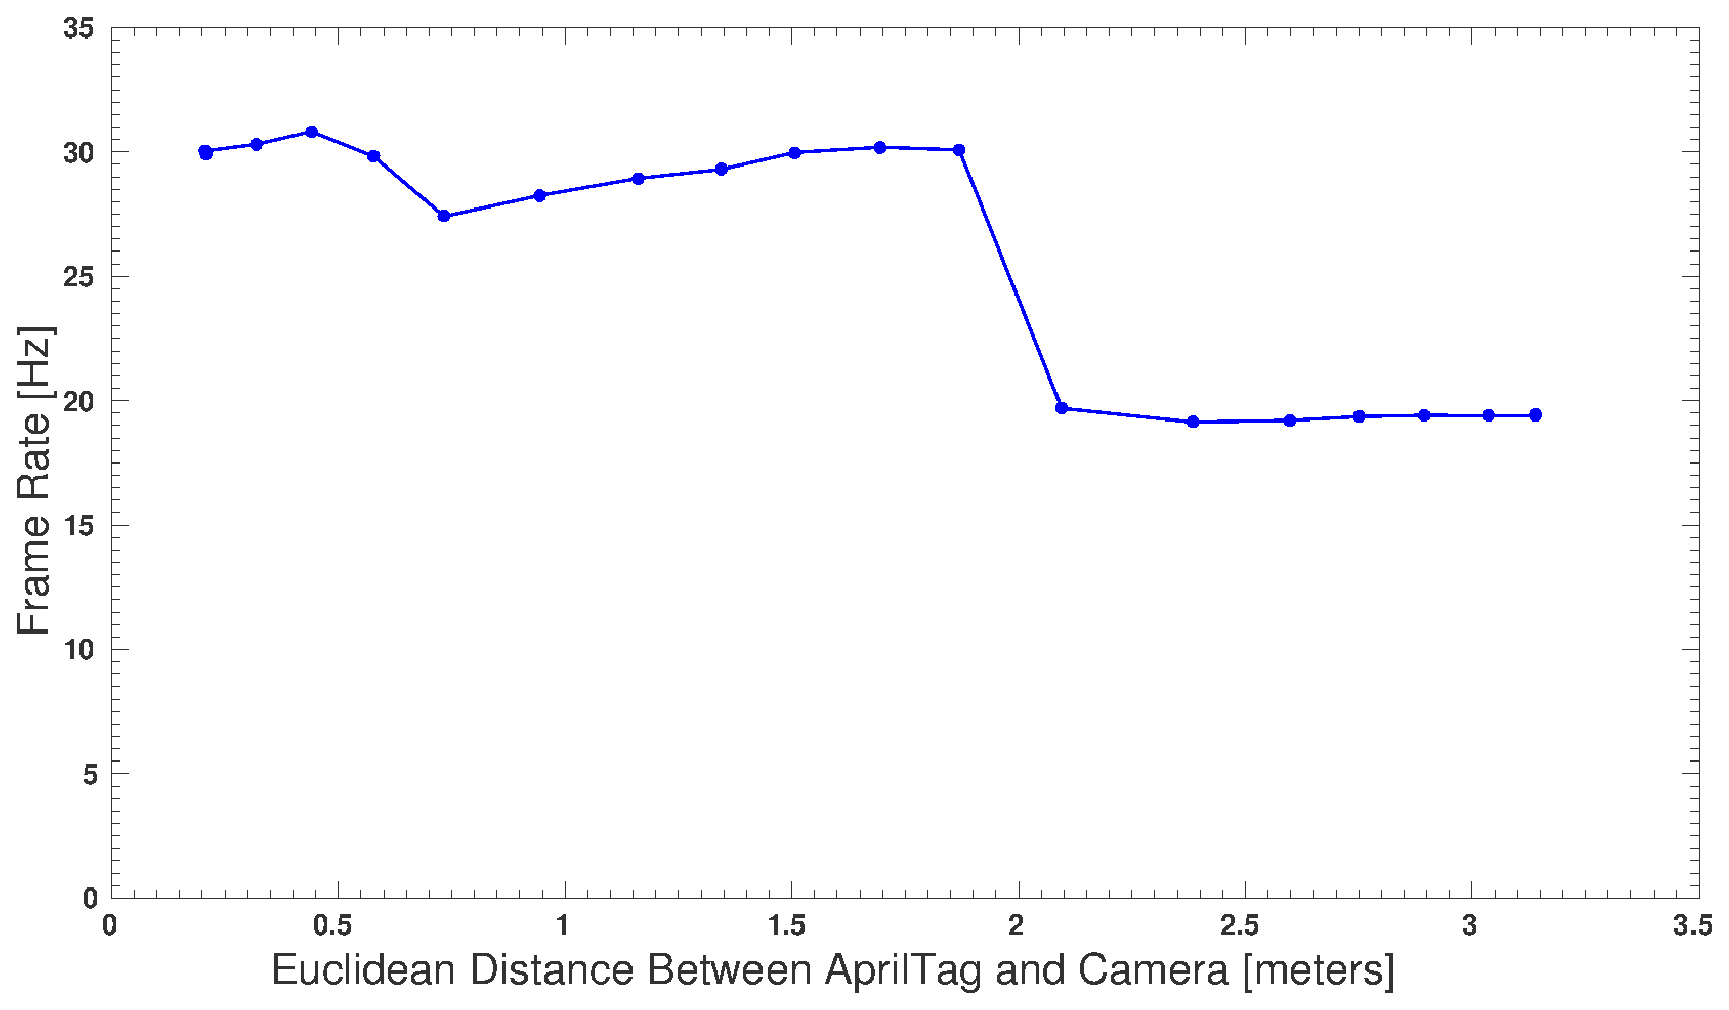
\includegraphics[width=\textwidth]{images/Apr_Distance_Error.eps}
		\caption{}
		
	\end{subfigure}
	\caption{Evaluation of AprilTag state estimation and update rate as functions of distance}
	\label{fig:AprilTag_eval}	
\end{figure}

From Figure \ref{fig:AprilTag_eval} it appears that the average error of the estimated euclidean distance compared to MOCAP ground truth is within approximately $\pm 20 cm$ for any measurements between 0 and 3 meters. Due to the limited range of the MOCAP system distances greater than 3 m between the camera and the AprilTag were not tested. The system was also able to maintain a frame rate of approximately 30 fps in cases camera is less then 2 meters away from the AprilTag while producing estimates with an error within approximately $\pm 0.05 cm$. In future, an analysis of the sources of error in Figure \ref{fig:AprilTag_eval} will be conducted as well as evaluation of the error as a function of angle between the AprilTag and the camera. 

It is suspected that the PointGrey Camera used in this test was not operating at the requested frame rate of 60 fps. This was not noted until after analysing the data and will be investigated this coming week. In the past there have been problems with the PointGrey camera changing its settings after several reboots, often resting the frame rate from 30 fps to 60 fps with no warning or indication. If this is the case, then the update rate of the AprilTag library on the Odroid may actually be faster than what is shown in Figure \ref{fig:AprilTag_eval}. In cases where a more powerful computer can be used, the adaptive image processing method results in the AprilTag library operating at 60 fps with no delay, making it extremely useful on machines that can leverage greater computational power. 

\subsection{PID and Controller Results}
The PID controllers derived in section \ref{subsec:position_controller} were tested on the quadrotor using the MOCAP system. Due to time constraints evaluation of the PID controller was only conducted using the MOCAP system to provide state estimates, but in the coming week further tests using the AprilTag system will be conducted. After a signifcant amount of testing the following values for the proportional, derivative and integral gains ($K_p, K_d, K_i$) were determined for the roll, pitch and height controllers. Using state information from the MOCAP system, the yaw of the quadrotor was fixed at zero degrees for all of the following tests. The commanded roll and pitch attitude commands produced by the PID controllers was also limited to $\pm 20^0$ for safety. 

\begin{center} 
	\vspace{-0.4cm}
	\begin{tabular}{l r}
		\hline
		\textbf{Roll Controller} \\
		\hline
		$K_{p}$ &  0.205 \\
		$K_{i}$ & 0.05 \\
		$K_{d}$ &  0.02 \\
		\\
		\hline
		\textbf{Pitch Controller} \\
		\hline
		$K_{p}$ & 0.205 \\
		$K_{i}$ & 0.05 \\
		$K_{d}$ & 0.02 \\
		\\
		\hline
		\textbf{Thrust Controller} \\
		\hline
		$K_{p}$ & 0.2 \\
		$K_{i}$ & 0.0 \\
		$K_{d}$ & 0.02 \\
	\end{tabular}
\end{center}

Figures \ref{fig:pid_roll_command} \ref{fig:pid_roll_error},	\ref{fig:pid_pitch_command}, \ref{fig:pid_pitch_error}, \ref{fig:pid_thrust_command}, \ref{fig:pid_thrust_error} highlight the PID position control signal (roll, pitch and thrust) and corresponding proportional, integral and derivative error components while a quadrotor was set to hover at $(0, 0, 1)$ for approximately 65 seconds. Large disturbances were applied manually to the hovering quadrotor with a testing apparatus (a plank of wood) to test the correction behaviour of the position controller implemented. These disturbances are applied at the 15, 21, 37, and 57 second marks in all six Figures. In the case of the elevation controller, there was no integral term used due to the risk of a suck throttle occurring in cases where the quadrotor did not detect landing and tack off correctly.

From Figures \ref{fig:pid_roll_command} and \ref{fig:pid_pitch_command}, when the quadrotor is perturbed by a disturbance in teh horizontal plane, the position controller is able recover and return to the set point within 2-4 seconds. A video of flight that produced the dataset shown in \ref{fig:pid_roll_command} and \ref{fig:pid_pitch_command} can be viewed \href{https://www.youtube.com/watch?v=v1QDdZ0LdMc&index=17&list=PLk5z6lLnKFd6BD9EXWa09hqf6SNQhn59R}{here}.

In all cases there was significant amount of noise on the derivative error term as highlighted in Figures \ref{fig:pid_roll_error}, \ref{fig:pid_pitch_error}, and \ref{fig:pid_thrust_error}. It is suspected that this large error is due to the small time step of 0.01 seconds used in the calculation of the derivative term which has side effect of greatly amplifying any noise in the MOCAP state estimations. In cases where the MOCAP measurement did not correctly correspond to the current true state of the vehicle large spikes can be noted which appears around the 9 second mark in Figures \ref{fig:pid_roll_error}, \ref{fig:pid_pitch_error}, and \ref{fig:pid_thrust_error}. The noise in the MOCAP system can be reduced by adding additional markers to the quad and by making a more rigid frame to mount the tracking markers. 

These plots also highlight the need to place a limit on the commanded output as in the roll and pitch PID controllers there were cases where the sum of the derivative term with the proportional and integral error terms may lead to a commanded pitch or roll greater than 60 degrees which is considered far to aggressive for the quadrotor used in these experiments. Further tuning and testing of the PID controller will be carried out in the coming weeks along with tests that do not require the yaw to be stabilized at zero degrees. Theoretically it will be possible to directly apply the PID controllers to state estimates obtained by the AprilTag directly and in such cases it should be possible to use these same controllers to follow and land on a moving AprilTag. Such a test will be the focus of the majority of effort in the coming weeks. 


\begin{figure*}
	\centering
	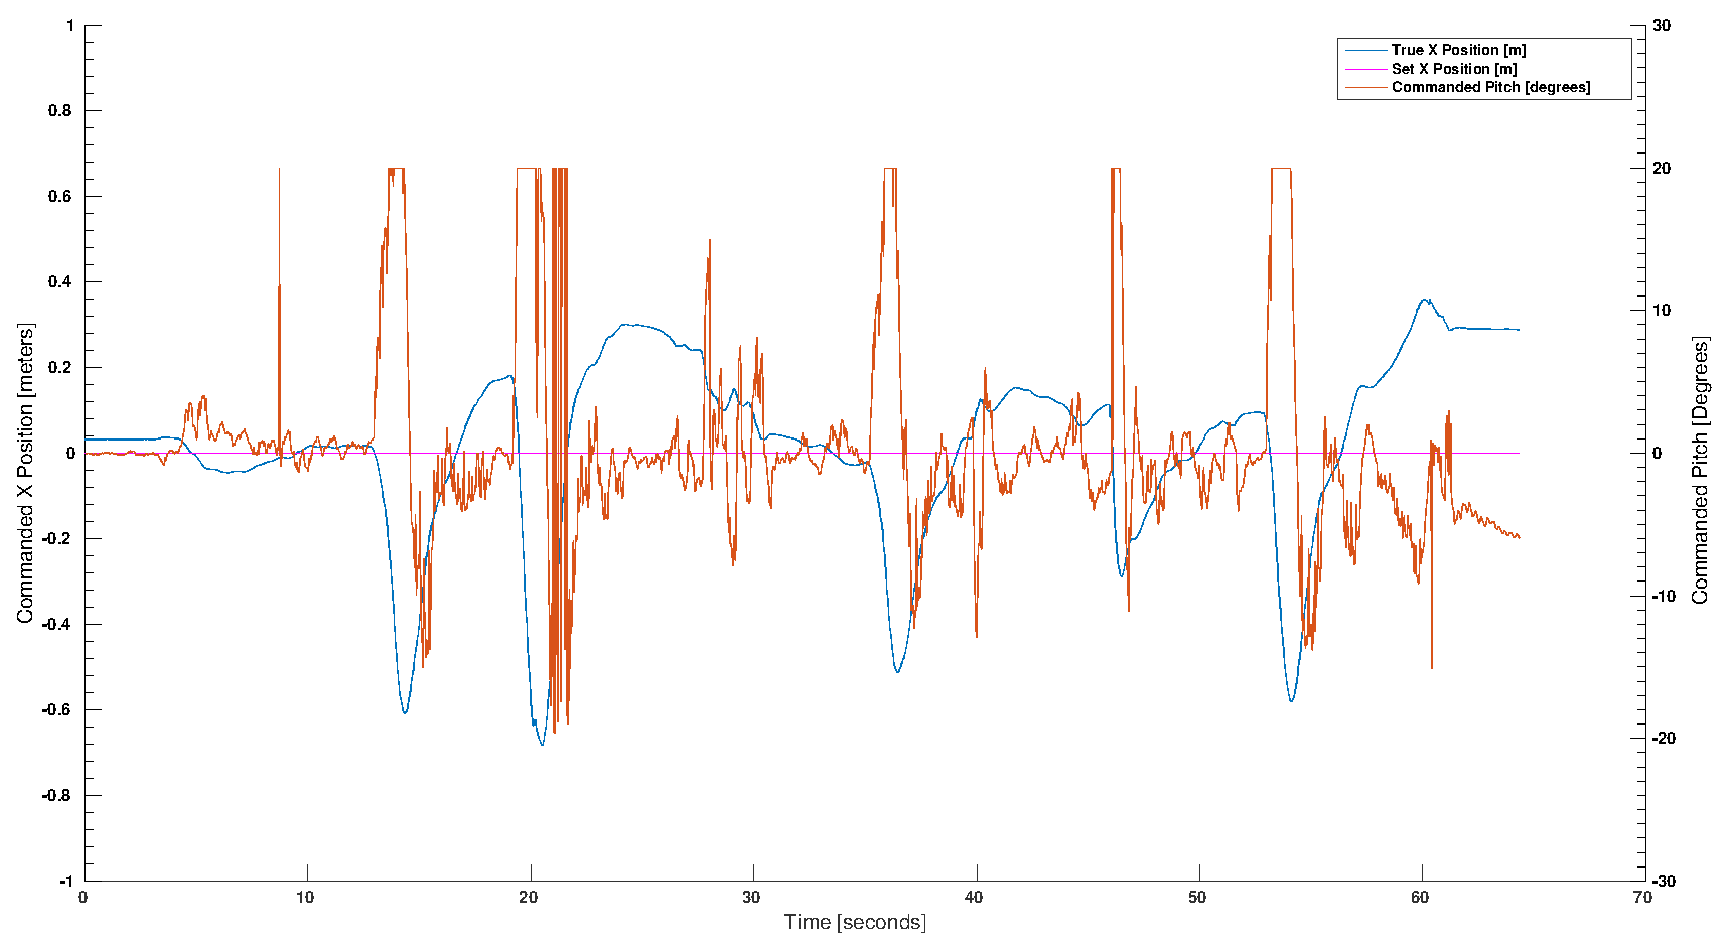
\includegraphics[width=\textwidth]{images/PID_Pitch_x_true_and_obs.eps}
	\caption{Position Controller - Pitch Command}
	\label{fig:pid_roll_command}
\end{figure*}

\begin{figure*}
	\centering
	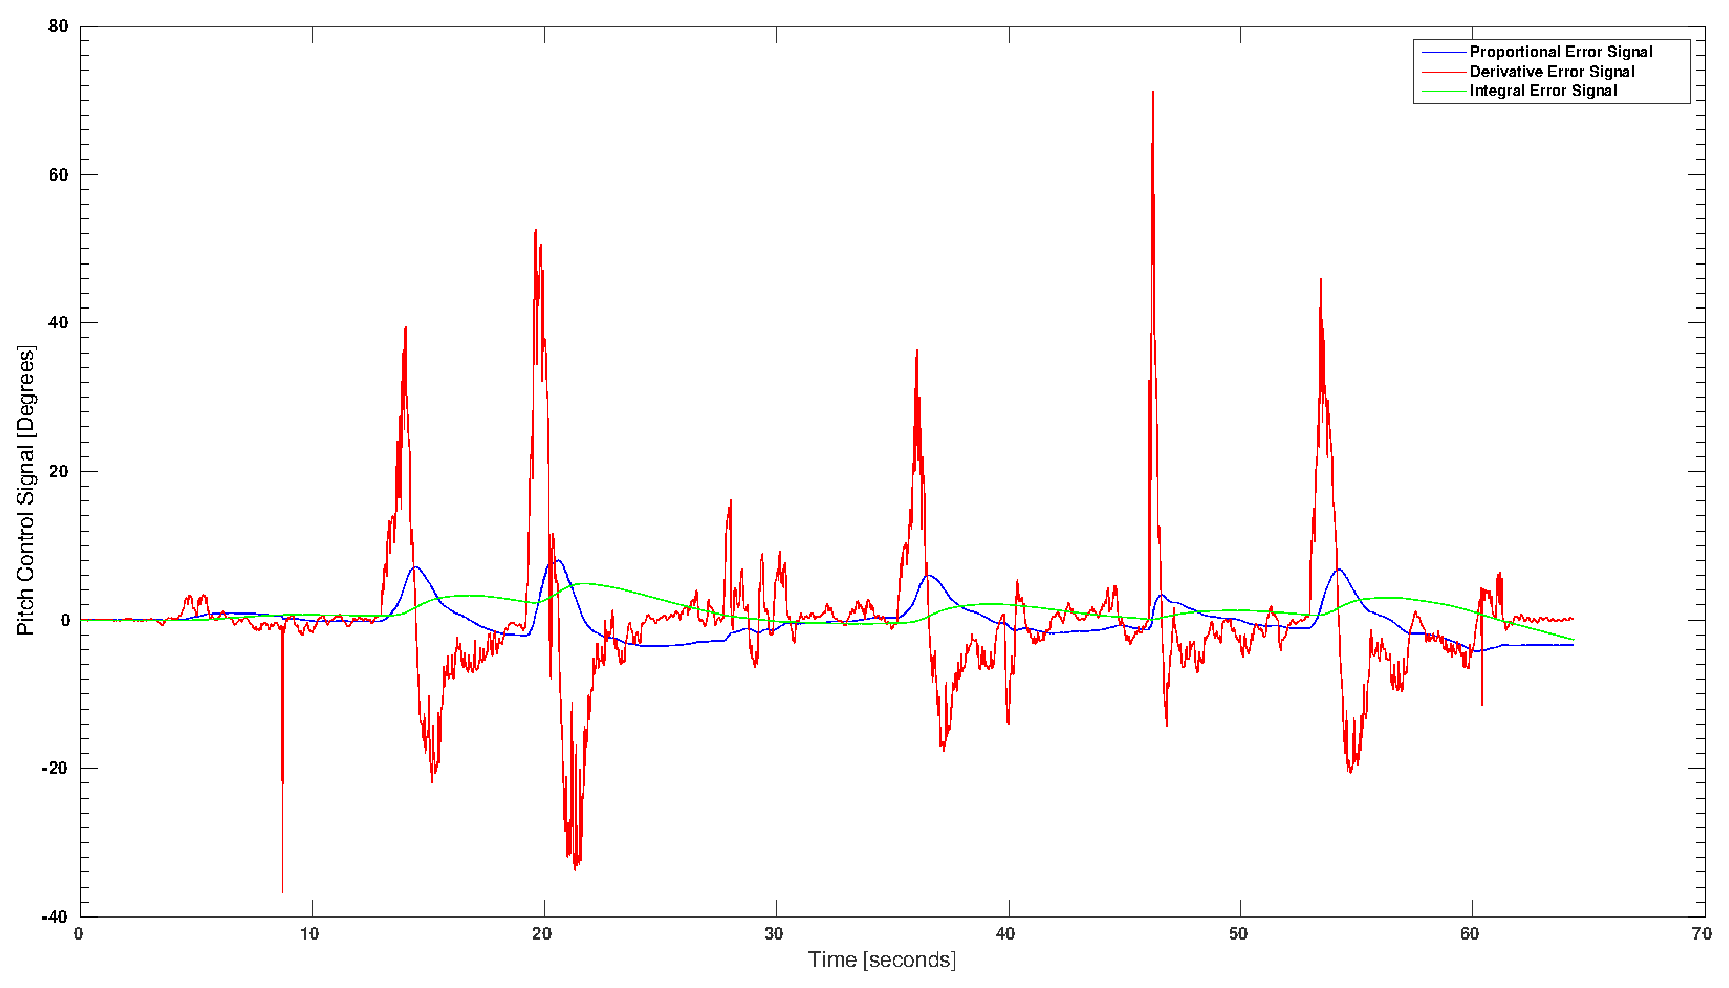
\includegraphics[width=\textwidth]{images/PID_Pitch_Controls.eps}
	\caption{Position Controller - Pitch Control Signal Components}
	\label{fig:pid_roll_error}
\end{figure*}

\begin{figure*}
	\centering
	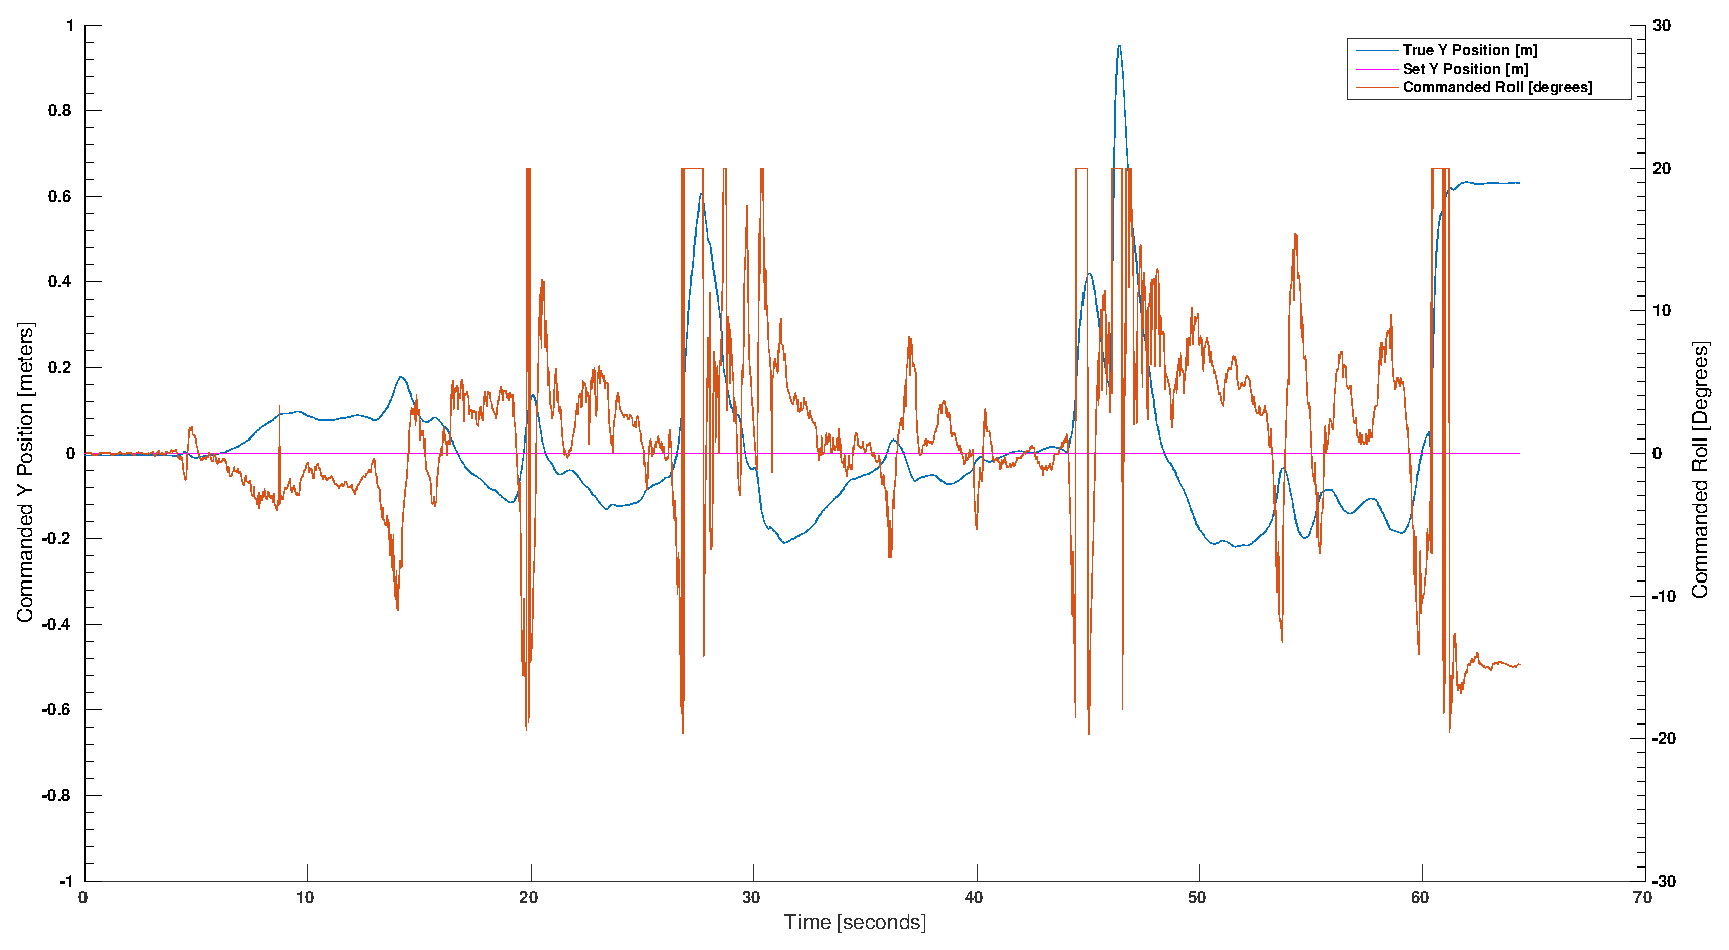
\includegraphics[width=\textwidth]{images/PID_Roll_y_true_and_obs.eps}
	\caption{Position Controller - Roll Command}
	\label{fig:pid_pitch_command}
\end{figure*}

\begin{figure*}
	\centering
	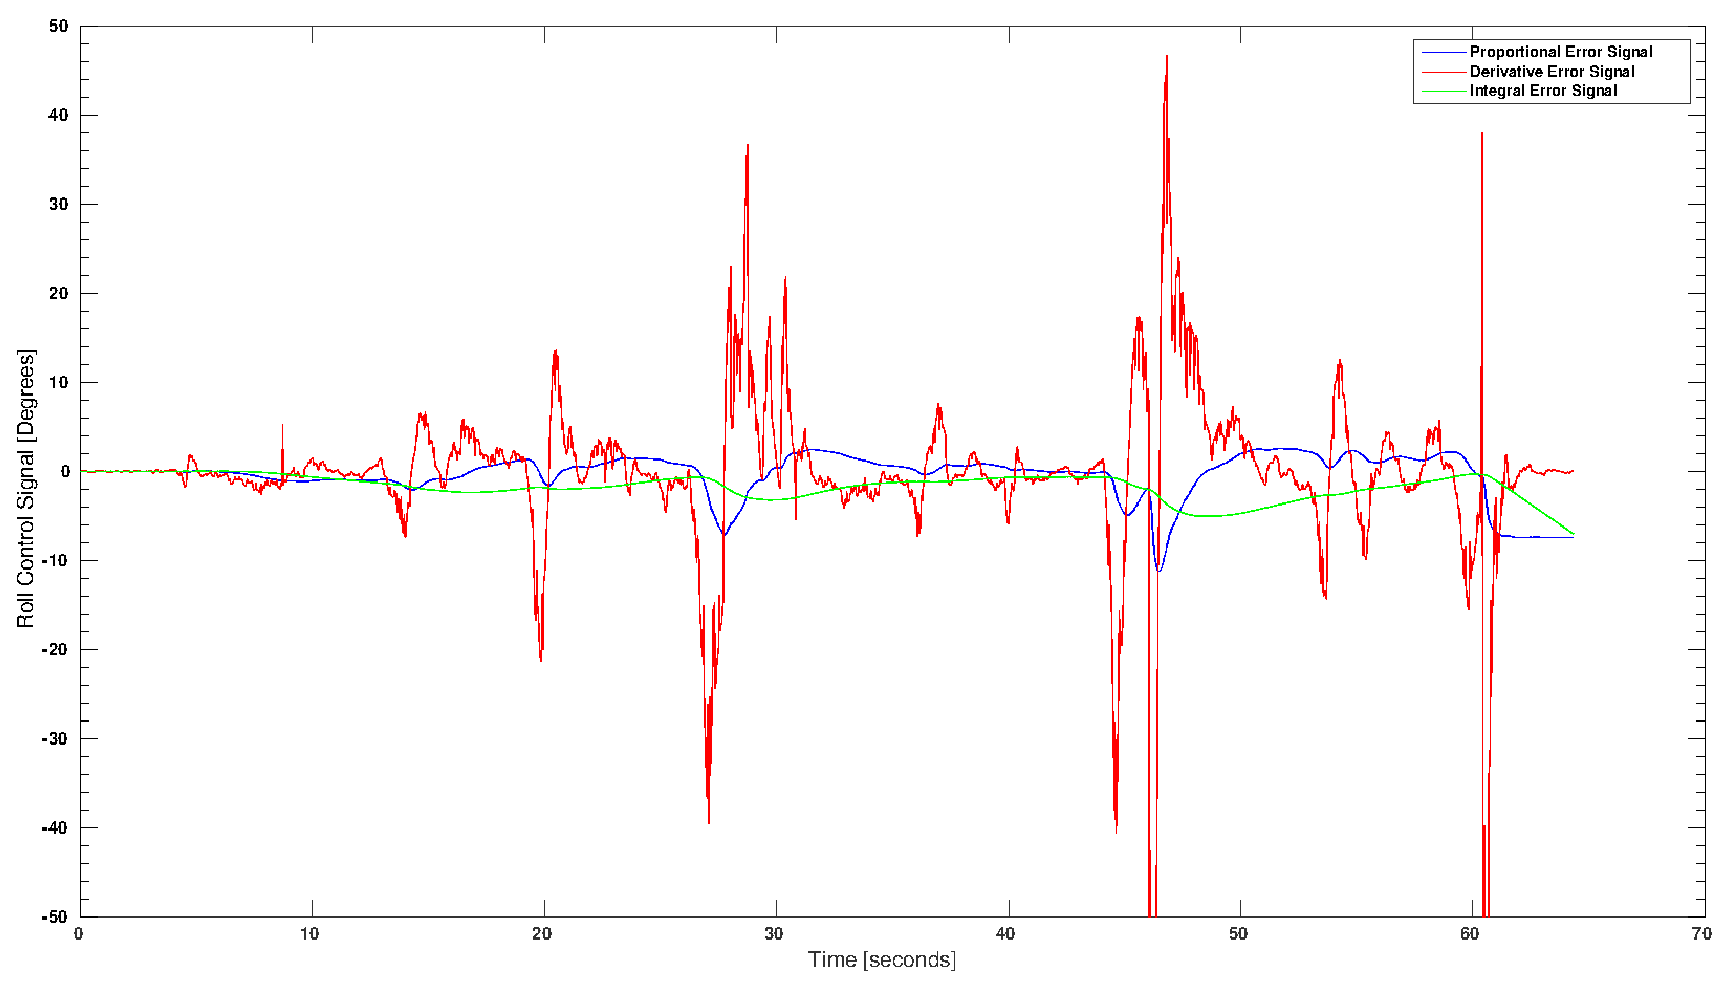
\includegraphics[width=\textwidth]{images/PID_Roll_Controls.eps}
	\caption{Position Controller - Roll Control Signal Components}
	\label{fig:pid_pitch_error}
\end{figure*}

\begin{figure*}
	\centering
	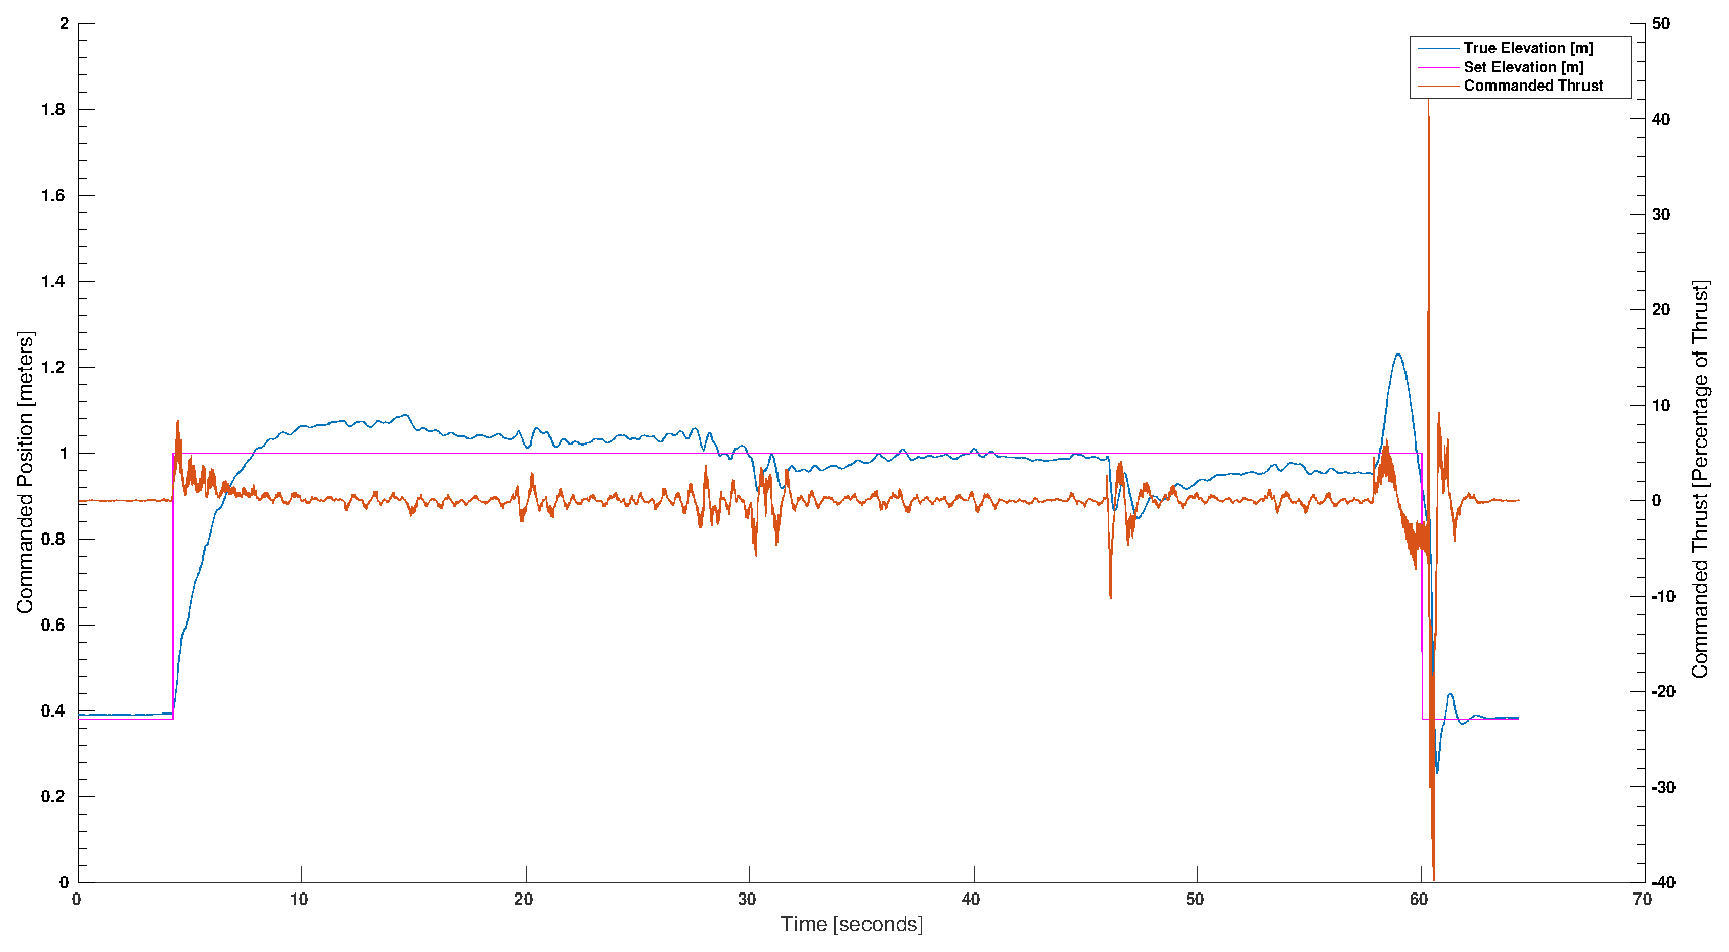
\includegraphics[width=\textwidth]{images/PID_Elevation_True_and_obs.eps}
	\caption{Position Controller - Thrust Command}
	\label{fig:pid_thrust_command}
\end{figure*}

\begin{figure*}
	\centering
	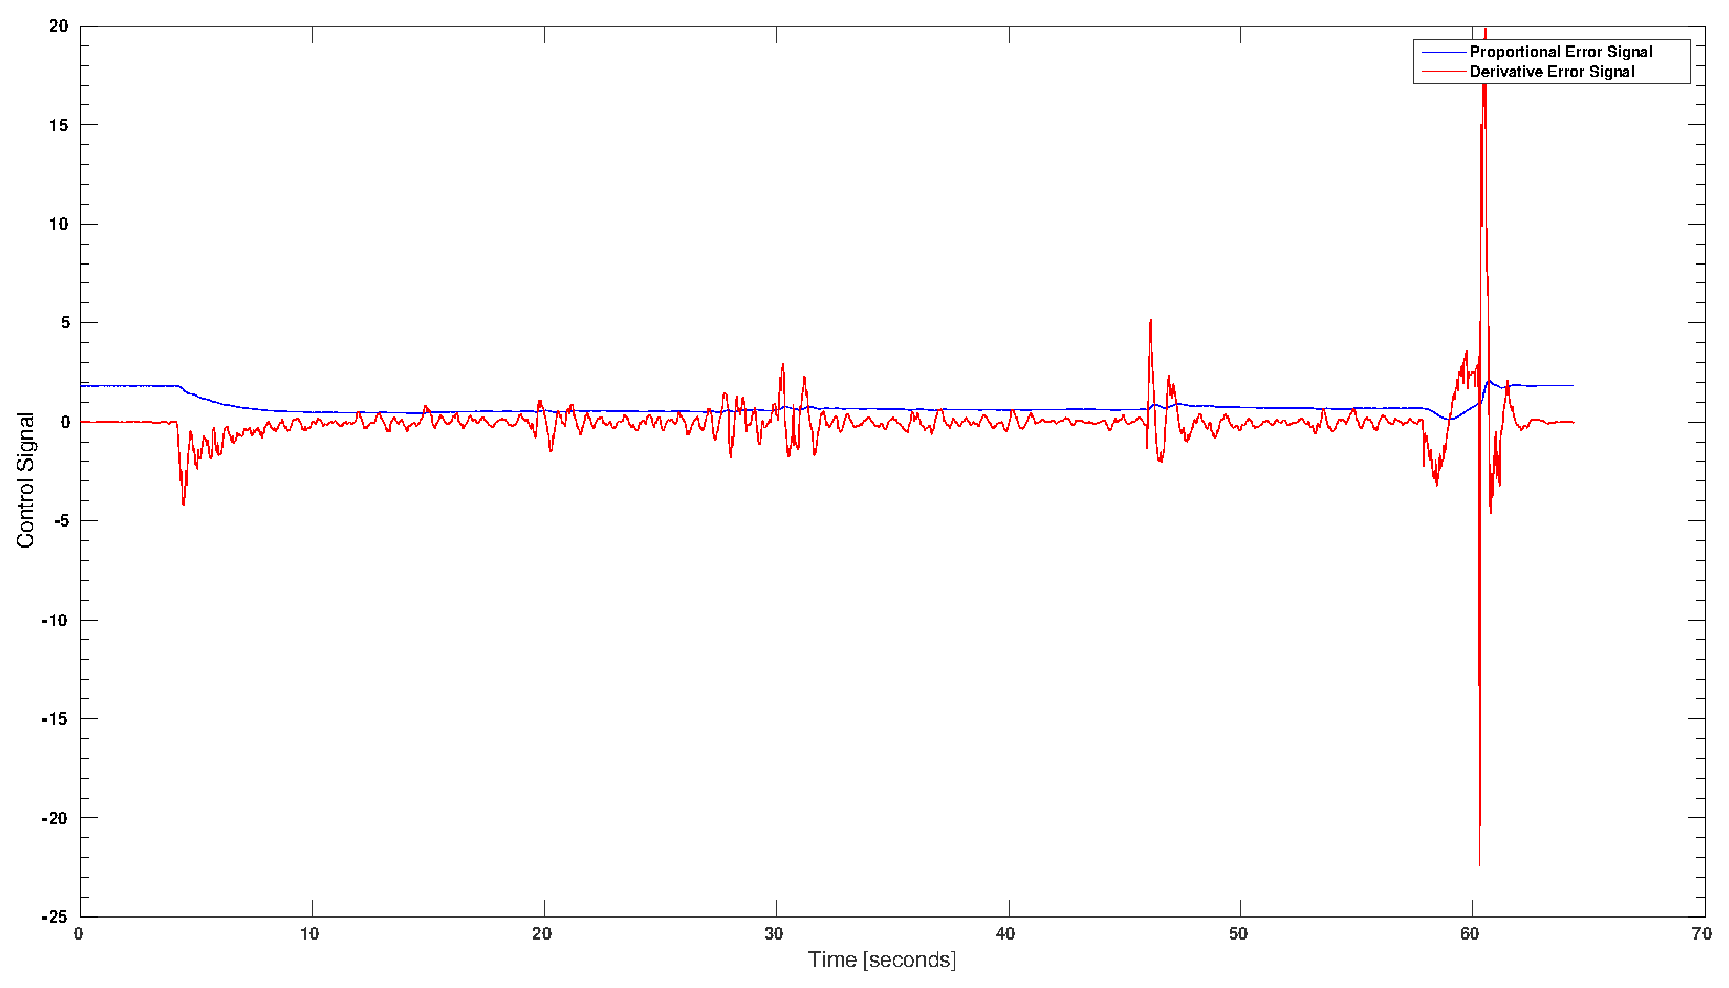
\includegraphics[width=\textwidth]{images/PID_Elevation_Controls.eps}
	\caption{Position Controller - Thrust Signal Components}
	\label{fig:pid_thrust_error}
\end{figure*}


\section{Conclusions and Future Work}
A set of algorithms were developed to provide fast, reliable and accurate estimations of state between a landing pad and a quadrotor using a series of image preprocessing methods and the MIT AprilTags library. These methods were tested and evaluated using a motion capture system to provide ground truth and were shown to provide update rates of greater than 20 Hz for a low power onboard, quadrotor mounted computer system. A set of PID controllers were developed, tested and evaluated using the same motion capture system to provide state estimates and a ground truth. A set of stable yet responsive PID gains were found and tested using this system and an evaluation of their behaviour in the presence of large disturbances was conducted. 

In the coming weeks the state estimates used by the PID controllers will be provided solely by an AprilTag located on the ground and a series of procedures using these controllers will be derived such that the quadrotor will hover over the AprilTag before initializing a landing procedure. Once such a landing can be performed consistently in the face of minor disturbances it, the same procedure will be applied to quadrotor and landing system where the landing platform will be mounted to a moving vehicle.

\bibliography{report}{}
\bibliographystyle{ieeetr}
\end{document}